\textbf{(a) Construct a continuous-data histogram of the service times (in ac.dat - Exercise 1.2.6).\\
(b) Compare the histogram mean and standard deviation with the corresponding sample mean and standard deviation, and justify your choice of histogram parameters $a$, $b$, and either $k$ or $\delta$.}\\\\
\noindent Terminal Output\\
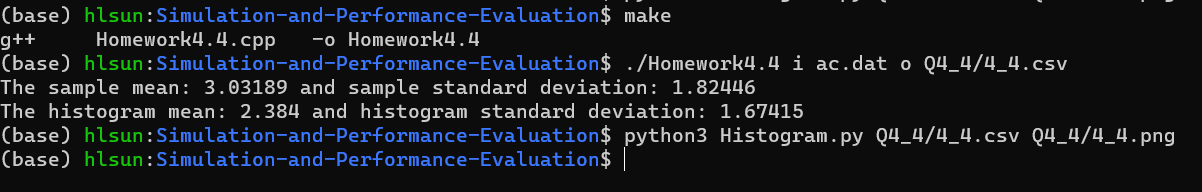
\includegraphics[scale=0.6]{Sections/Q4/4_4_terminal.png}\\

\noindent The sample mean: 3.03\\
The sample standard deviation: 1.82\\
The histogram mean: 3.03\\
The histogram standard deviation: 1.81\\\\

\noindent We can see that the sample and histogram mean and standard deviation are similar. This means that the number of bins used was sufficient to ensure an accurate representation of the data. Additionally, the histogram is mostly smooth, meaning the number of bins used was not excessively high in order to achieve this sample statistic performance. \\\\

\noindent a and b were chosen to be the minimum and maximum values, as this allows the histogram to fit all of the data while also not allocating bins for data outside the range. The number of bins was chosen such that $k \in [\lfloor ln(n) \rfloor, \lfloor\sqrt{n}\rfloor]$. Given that $n = 500$, $k \in [6,22]$. 18 was chosen because more bins than the minimum were needed knowing that outlier data is significantly larger than the mean. This can been seen in the histogram below, where there are several empty bins before reaching the maximum bin. However, setting $k$ too high, such as $k=22$ would result in a noisy histogram. Therefore, it was decided that $k=18$.\\\\

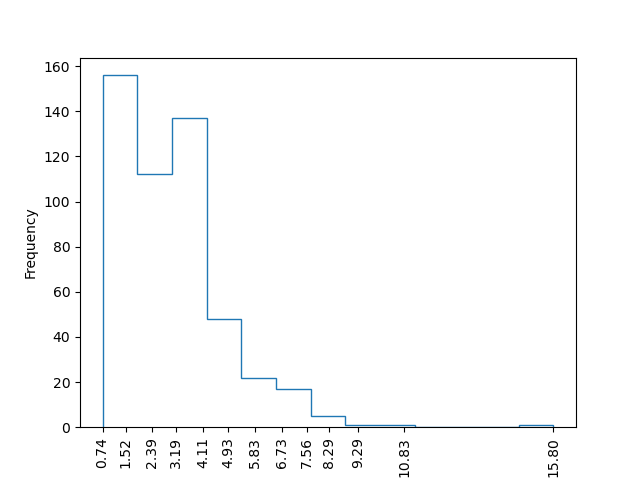
\includegraphics[scale=1]{Sections/Q4/4_4.png}
\newpage
\begin{lstlisting}[style=CStyle]
/**
 * Harrison Sun (sun.har@northeastern.edu)
 * EECE 5643 - Simulation and Performance Evaluation
 * Homework 4.4
 */

#define DEFAULT_IFILE		"ac.dat"
#define DEFAULT_OFILE		"output.txt"

#include <algorithm>
#include <cstdlib>
#include <cstring>
#include <fstream>
#include <stdio.h>
#include <exception>
#include <iostream>
#include <list>
#include <math.h> 
#include <string>
#include <vector>
#include "c_lib/rvgs.h"
#include "c_lib/rngs.h"
#include "checkarg/checkarg.h"

void sortDataIntoBins(const std::vector<double>& data, int numBins, std::vector<std::pair<double, long>>& meanOfBinAndCount) {
	// Initialize the meanOfBinAndCount vector with empty bins and counts of 0
	meanOfBinAndCount.clear();
	for (int i = 0; i < numBins; i++) {
		meanOfBinAndCount.push_back(std::make_pair(0.0, 0));
	}

	// Find the range of the data
	double minData = *std::min_element(data.begin(), data.end());
	double maxData = *std::max_element(data.begin(), data.end());
	double range = maxData - minData;

	// Calculate the width of each bin
	double binWidth = range / numBins;

	// Sort the data into bins and update the mean and count of each bin
	for (int i = 0; i < data.size(); i++) {
		// Determine which bin the data point belongs to
		int binIndex = std::min(static_cast<int>((data[i] - minData) / binWidth), numBins - 1);

		// Update the mean and count of the bin
		double binMean = meanOfBinAndCount[binIndex].first;
		long binCount = meanOfBinAndCount[binIndex].second;
		binMean = (binMean * binCount + data[i]) / (binCount + 1);
		binCount++;
		meanOfBinAndCount[binIndex] = std::make_pair(binMean, binCount);
	}
}



/**
 * int main() - The main function
 *
 * @param int argc - the number of arguments
 * @param char* argv[] - the arguments
 *
 * @return 0 if the program runs successfully
 * 
 * This is the main function. It reads in a data file in tab separated format. The first column contains the arrival times and the second column
 * contains departure times.
 * 
 */

int main(int argc, char* argv[])
{
	// Create two vectors to store the data
	std::vector<double> arrival_times{};
	std::vector<double> departure_times{};
	std::vector<double> service_times{};

	// Histogram Parameters
	int nHistogram { 500 }; // The number of jobs in the data file
	// The number of bins in the histogram. Ideally, k ~ [ln(n), sqrt(n)] => Choosing from k ~ [6, 22]
	
	/*****************************************************************************************************************************************************************

		The number of bins is chosen to be 18 This is significantly larger than the minimum k = 6. The reason for this choice is that the service times are empirical 
		data and may have significant outliers that would not fit well with other data when given too few bins. However, 22 bins would be too many, as the data has
		high variance and would thus have a lot of empty bins. 18 bins is a good compromise between the two.
		
	*****************************************************************************************************************************************************************/
	
	int nBins{18};
	
	// File names
	std::string inputFileName{};
	std::string outputFileName{};

	// Set the input file stream
	for (int i = 0; i < argc; ++i)
	{
		if (*argv[i] == 'i')
		{
			inputFileName = argv[i + 1];
			break;
		}
		else
		{
			inputFileName = DEFAULT_IFILE;
		}
	}
	
	// Set the output file stream
	for (int i = 0; i < argc; ++i)
	{
		if (*argv[i] == 'o')
		{
			outputFileName = argv[i + 1];
			break;
		}
		else
		{
			outputFileName = DEFAULT_OFILE;
		}
	}
	
	double arrival_time{};
	double departure_time{};
	
	std::ifstream infile;
	infile.open(inputFileName.c_str());
	
	// Read in the data from the tsv to the vectors
	while (infile >> arrival_time >> departure_time)
	{
		arrival_times.push_back(arrival_time);
		departure_times.push_back(departure_time);
	}
	infile.close();
	
	// Calculate the service times and store them in the service_times vector
	for (int i = 0; i < arrival_times.size(); ++i)
	{
		// Check if the service node is free at arrival
		if (arrival_times[i] > departure_times[i - 1])
		{
			service_times.push_back(departure_times[i] - arrival_times[i]);
		}
		// If the job has to wait in a queue, the service starts after the previous job is finished
		else
		{
			service_times.push_back(departure_times[i] - departure_times[i - 1]);
		}
	}

	// Calculate the total service time
	double total_service_time{};
	for (std::vector<double>::iterator i = service_times.begin(); i != service_times.end(); ++i)
	{
		total_service_time += *i;
	}
	
	// Calculate the sample mean and standard deviation
	double sample_mean{ total_service_time / service_times.size() };
	double sample_std{};
	
	// Standard Deviation
	for (std::vector<double>::iterator i = service_times.begin(); i != service_times.end(); ++i)
	{
		sample_std += pow(*i - sample_mean, 2);
	}
	sample_std = sqrt(sample_std / (service_times.size() - 1));

	// Vector to store the bin information as a pair
	std::vector<std::pair<double, long>> BinVector;

	// Call the function to sort the data into bins
	sortDataIntoBins(service_times, nBins, BinVector);

	// Store the bin means and counts in output file
	std::ofstream outfile;
	outfile.open(outputFileName.c_str());
	
	for (int i = 0; i < nBins; ++i)
	{
		outfile << BinVector[i].first << ", " << BinVector[i].second << std::endl;
	}
	
	outfile.close();
	
	// Calculate the histogram mean and standard deviation
	double histogram_mean{};
	double histogram_std{};
	
	for (int i = 0; i < nBins; ++i)
	{
		histogram_mean += BinVector[i].first * BinVector[i].second;
	}
	
	histogram_mean /= nHistogram;
	
	for (int i = 0; i < nBins; ++i)
	{
		histogram_std += BinVector[i].second * pow(BinVector[i].first - histogram_mean, 2);
	}
	
	histogram_std = sqrt(histogram_std / (nHistogram - 1));
	
	// Output the means and standard deviations
	std::cout << "The sample mean: " << sample_mean << " and sample standard deviation: " << sample_std << std::endl;
	std::cout << "The histogram mean: " << histogram_mean << " and histogram standard deviation: " << histogram_std << std::endl;
	return 0;
}
\end{lstlisting}